\chapter{SpreadRank}
\label{chp:spreadrank}

The previous algorithm, DOSRank, calculated the amount of flows.
While a large amount of flows may indicate that something is wrong,
 it may also simply indicate a very active node.
This chapter proposes SpreadRank, an algorithm to find hosts that are standing out due to the spreading they are causing.
SpreadRank calculates how far connections spread.
Spreading as an anomaly is described in chapter~\ref{chp:anomalies}.


\section{Overview of algorithm}
This thesis proposes SpreadRank, an algorithm to determine how far similar traffic spreads over hosts.
\emph{depth} in SpreadRank is defined in equation~\ref{eq:spreadrank1} and illustrated in figure~\ref{fig:spreadrank}.
The value of $d$ is the longest path from a host initiating a connection to another host receiving a similar connection.
\emph{spreading} in SpreadRank is defined in equation~\ref{eq:spreadrank2} and illustrated in figure~\ref{fig:spreadrank}.
The value of $s$ is the sum of all neighbours' $d$ value, plus the amount of neighbours.
Another way of looking at SpreadRank, is that during the first superstep, all nodes will send a token in the opposite direction of the flow.
This token contains the timestamp from the flow.
During all subsequent steps, all nodes that have received a token will send tokens again, but \emph{only to flows that have a lower timestamp than the token}.
\emph{Depth} is then defined as the last superstep during which tokens were received, and \emph{spread} is defined as the total amount of tokens received.


\begin{figure}[h]
	\caption{Small example graph with results of one node, all nodes are hosts}
	\label{fig:spreadrank}
	\centering
		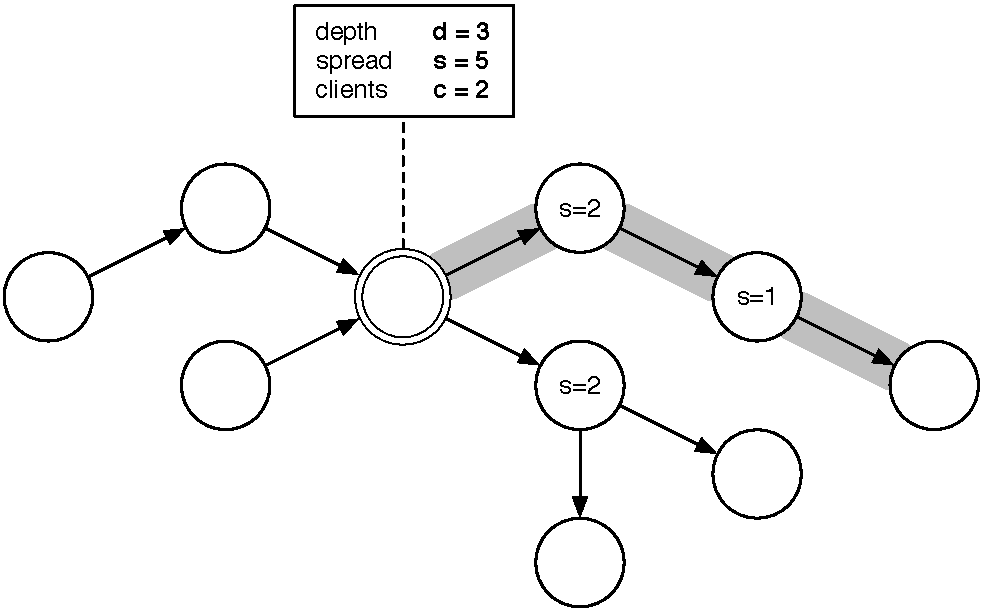
\includegraphics[width=0.75\textwidth]{spreadrank}
\end{figure}
\begin{equation}
	\label{eq:spreadrank1}
	d(x) = 1 + \max_{y \in N^{-}(x)} d(y).
\end{equation}
\begin{equation}
	\label{eq:spreadrank2}
	\displaystyle s(x) = \sum_{y \in N^{-}(x)} d(y) + \left\vert{N^{-}(x)}\right\vert.
\end{equation}
\emph{Where $E$ is the set of all edges in the graph, $f(x)$ and $f(y)$ are vertex values and $N^{-}(x)$ is a set of all incoming edges from vertex $x$.}



SpreadRank bears similarities to Google's PageRank~\cite{page1999pagerank}.
Both algorithms use a graph model where vertices and edges represent real-world elements.
PageRank's model consists of web pages and hyperlinks and
 SpreadRank's model consists of services and flows.
Both algorithms calculate values for vertices based on how they are connected to other vertices.
The algorithms do, however, calculate different things,
 and as such use different metrics for calculating vertex values.
This is most apparent in that in PageRank vertices send each other part of their current score,
 while in SpreadRank vertices simply send the timestamp of a flow start.
This is because time is not important in PageRank; it does not matter who made a link first,
 while for SpreadRank it is important to know when a flow occurred,
 as spreading must occur in chronological order.


\section{OSI model}
The \gls{network layer} provides stateless communication between hosts, and can be used to observe which hosts communicate with each other by means of IP addresses.
Additionally, the IP header contains a protocol number, which gives some rough idea of the type of service.
The transport layer (layer 4) provides end-to-end communication, and can be used to observe what kind of services are being used, by looking at the protocol header.
Internet traffic consists mostly of TCP traffic, which makes TCP port numbers an interesting thing to look at.
SpreadRank only looks at TCP traffic, and assumes that identical port numbers indicate identical types of service.

SpreadRank must not be confused with the Dijkstra algorithm~\cite{dijkstra1959note},
 which can be used by layer 3 devices to find the shortest path between hosts.
SpreadRank operates on NetFlow data, which contains IP addresses of hosts and port numbers, which is layer 4 data.
The path that is observed is not a path via internet routers, but a path of hosts imitating each others behaviour.


\section{Data types}
\label{sec:data-types}
In the SpreadRank algorithm proposed in this thesis,
 IP-address and port number tuples are represented by vertices (figure~\ref{fig:datatype-spreadrank-vertex-id}).
The choice for this combination is due to \gls{spreading} occurring over the same port, which is the best NetFlow metric available to indicate type of traffic.
The vertex's value (figure~\ref{fig:datatype-spreadrank-vertex-value}) contains how far the traffic reaches (\gls{depth}) and how far their traffic spreads (\gls{spreading}).
Flows are represented by edges.
The edge has the flow start timestamp as value (figure~\ref{fig:datatype-spreadrank-edge}).


\begin{figure}[h]
	\caption{Data type of a SpreadRank vertex ID}
	\label{fig:datatype-spreadrank-vertex-id}
	\centering
		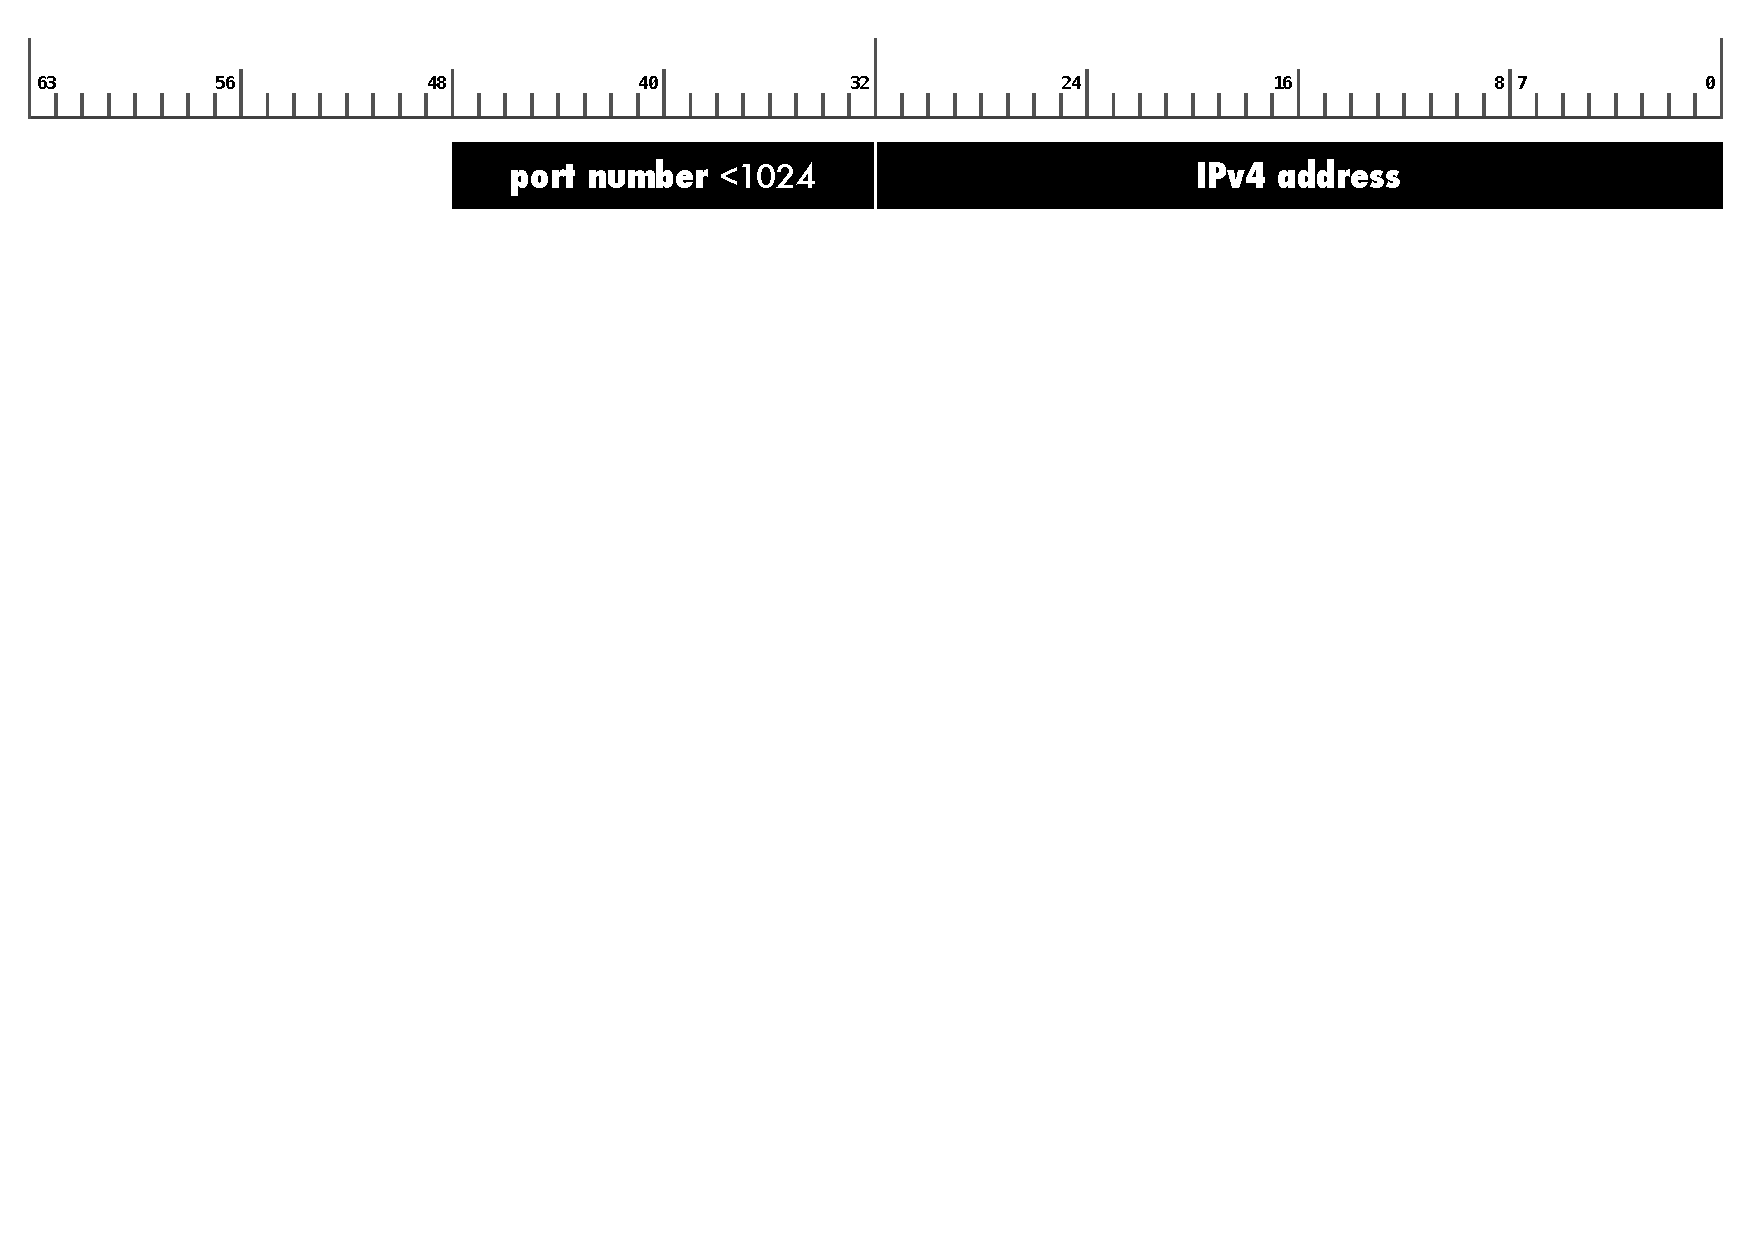
\includegraphics[width=1\textwidth]{datatype-spreadrank-vertex-id}
\end{figure}
\begin{figure}[h]
	\caption{Data type of a SpreadRank edge}
	\label{fig:datatype-spreadrank-edge}
	\centering
		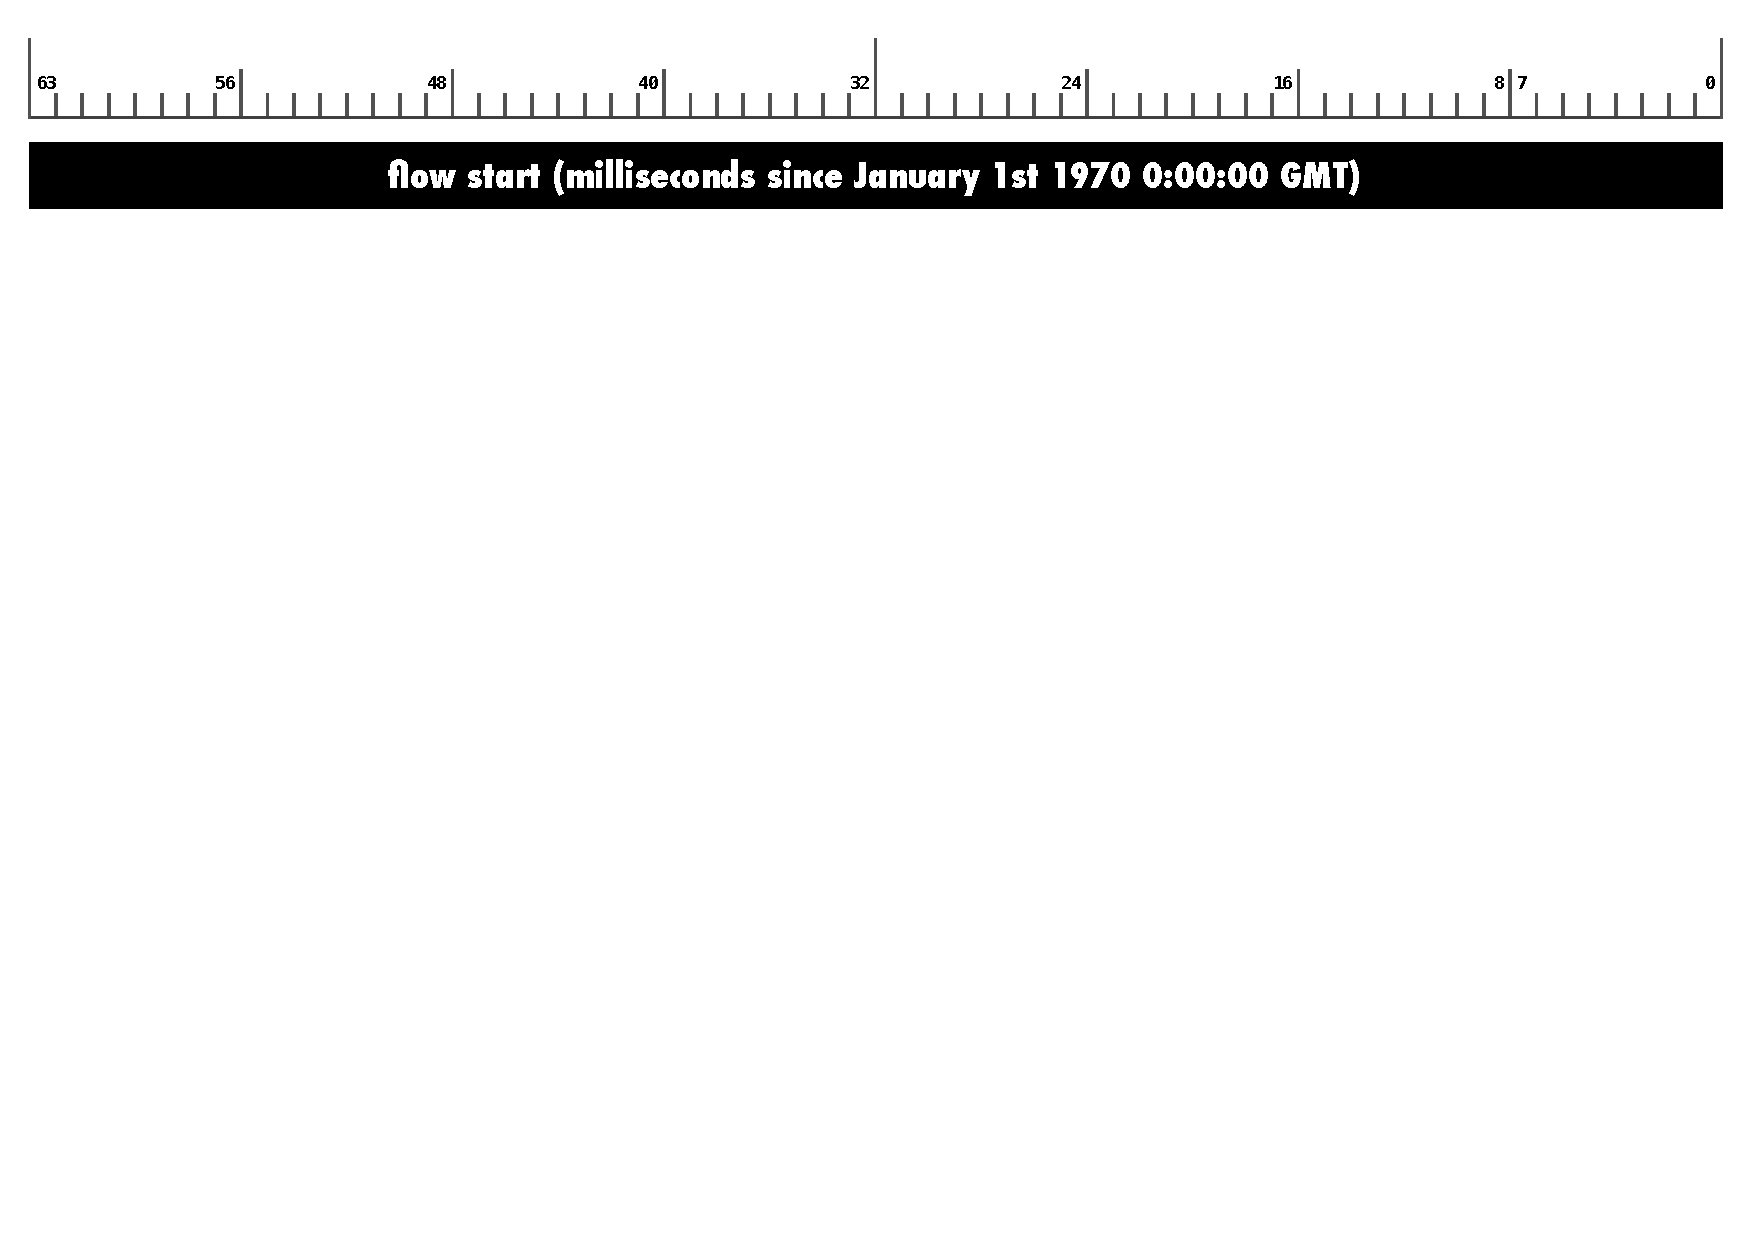
\includegraphics[width=1\textwidth]{datatype-spreadrank-edge}
\end{figure}
\begin{figure}[h]
	\caption{Data type of a SpreadRank vertex value}
	\label{fig:datatype-spreadrank-vertex-value}
	\centering
		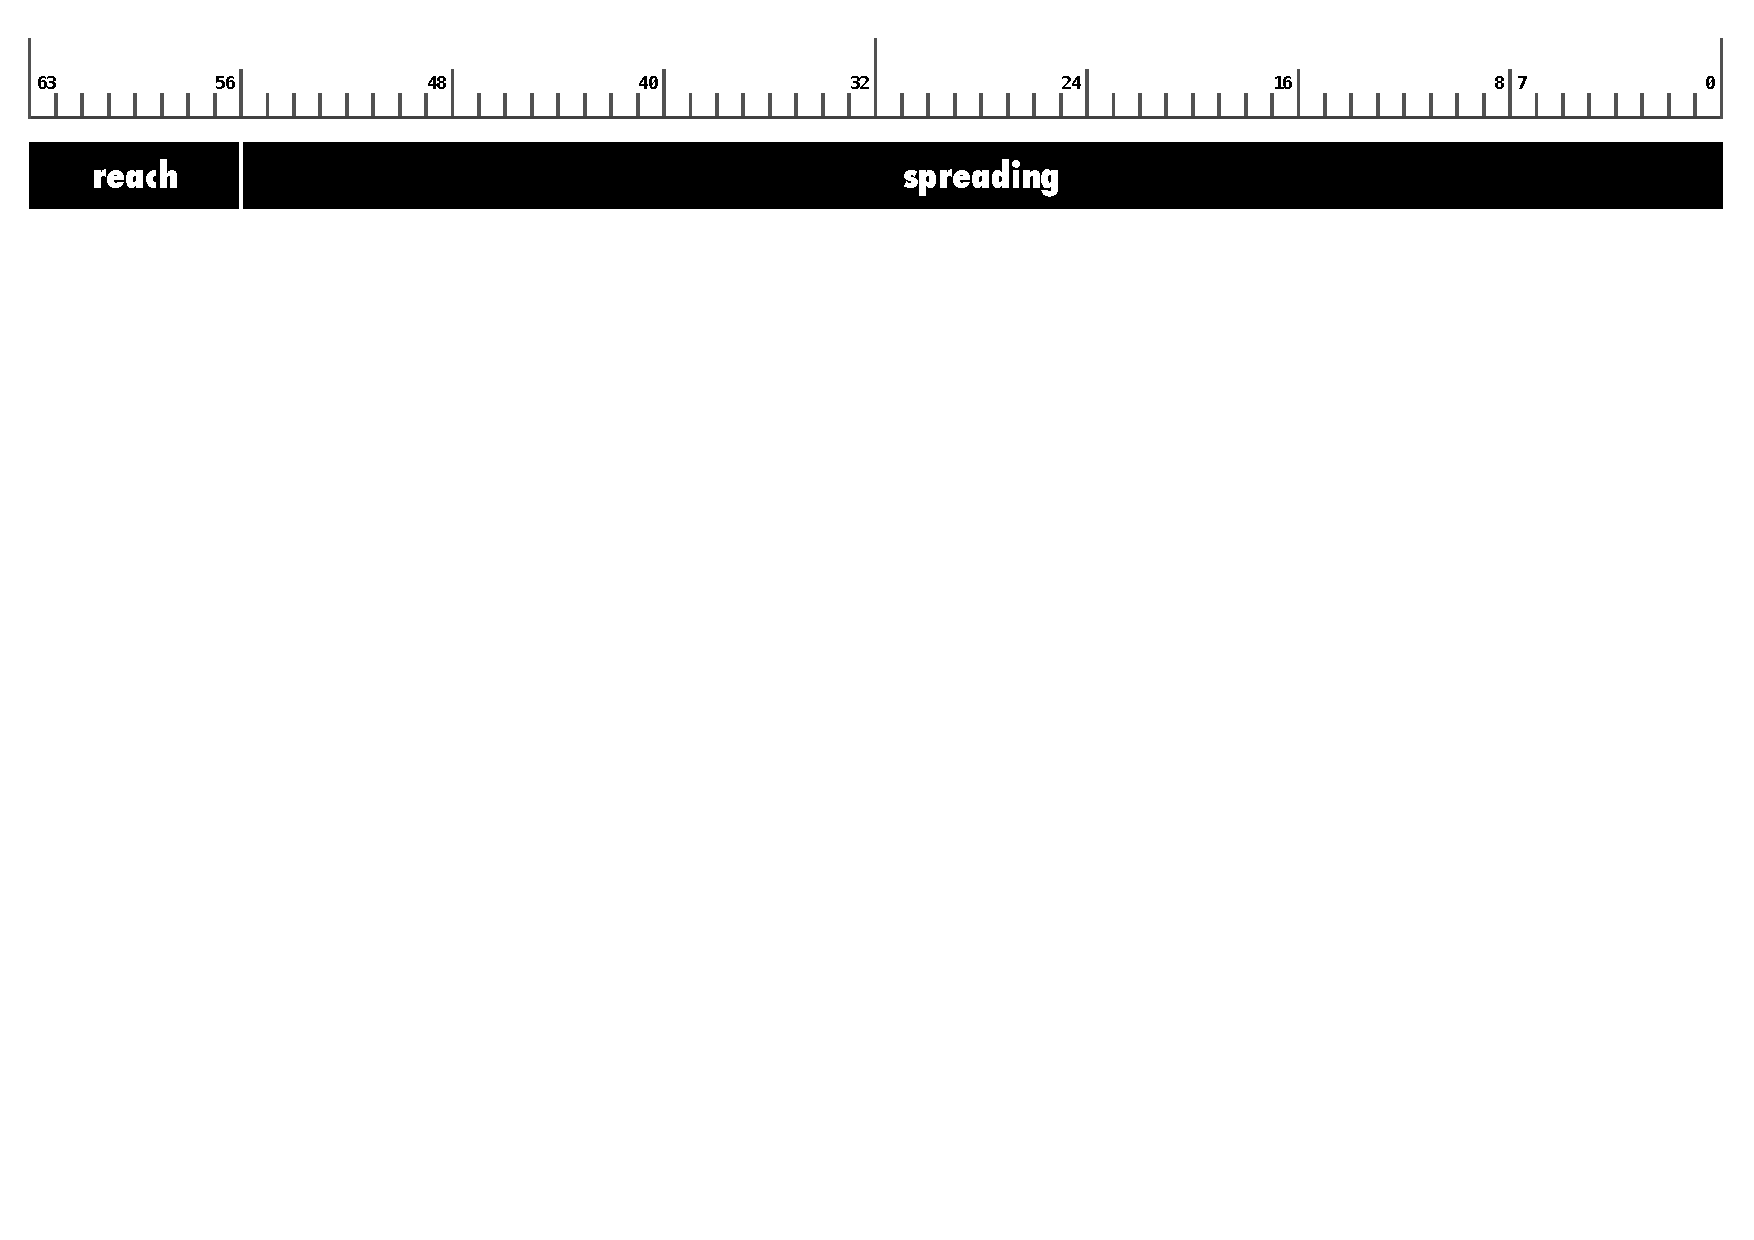
\includegraphics[width=1\textwidth]{datatype-spreadrank-vertex-value}
\end{figure}


\subsection{Filtering}
\label{sec:filtering}
Before calculation, all flows that do not represent a TCP or UDP connection are removed,
 as well as every flow not between a \gls{contact port} and an \gls{ephemeral port}.
Since the difference between a \gls{contact port} and an \gls{ephemeral port} may be vague,
 a \gls{contact port} is assumed to be a \gls{well-known port}, which is any port number below 1024~\cite{rfc1700}.
Any port from 1024 and up is assumed to be an \gls{ephemeral port}.
Different operating systems use different port numbers as \gls{ephemeral port}s,
 but no operating system uses ports under 1024 as \gls{ephemeral port}s (section~\ref{sec:conversion}).

Additionally, all double flows are removed, which means that there are always zero, one or two flows between two edges (no flows, one-directional, bi-directional).
For every vertex-pair, for every direction, the oldest edge is retained.
Since each edge has a timestamp as value, the edge with the lowest value is retained and edges with higher values are removed.


\subsection{Loop protection}
The removal of redundant edges is to provide a loop protection mechanism.
In a graph system, it is difficult to detect loops;
During calculation, only information about the vertex itself is known (outgoing edges, vertex id, vertex value, incoming messages).
It is not viable to include a trail of previous edges to the messages that are exchanged after the calculation;
 this would be expensive in terms of memory.

In the specific case of SpreadRank, this problem can be solved by only considering the first time a flow has been observed,
 and to ignore all subsequent occurrences (figure~\ref{fig:sequence1}).
If a host initiated a type of connection before it ever received it, it certainly did not initiate these connections because of the connection it received,
 and it is not a case of spreading (figure~\ref{fig:sequence2}).
Multiple hosts can initiate a connection before spreading occurs, in which case it is assumed that both are responsible (figure~\ref{fig:sequence3} and~\ref{fig:sequence5}).
It is possible that spreading is incorrectly assumed due to the log not observing a previous connection (figure~\ref{fig:sequence4}).
This can for example happen when logging started after the second host initiated a connection, but before the first host did.

\begin{figure}[h]
	\caption{Removal of duplicate flows}
	\label{fig:sequence1}
	\centering
		\includegraphics[width=0.5\textwidth]{sequence1}
\end{figure}
\begin{figure}[h]
	\caption{Spreading can only occur in sequence}
	\label{fig:sequence2}
	\centering
		\includegraphics[width=0.5\textwidth]{sequence2}
\end{figure}
\begin{figure}[h]
	\caption{Spreading with two clients and one server}
	\label{fig:sequence3}
	\centering
		\includegraphics[width=0.5\textwidth]{sequence3}
\end{figure}
\begin{figure}[h]
	\caption{Spreading with two clients and two servers}
	\label{fig:sequence5}
	\centering
		\includegraphics[width=0.5\textwidth]{sequence5}
\end{figure}
\begin{figure}[h]
	\caption{False positive spreading}
	\label{fig:sequence4}
	\centering
		\includegraphics[width=0.5\textwidth]{sequence4}
\end{figure}

\begin{equation}
	\label{eq:spreading}
	S = T_{\text{firstReceived}} < T_{\text{firstSent}}
\end{equation}


\section{Implementation}
\label{sec:implementation}
In Giraph, it is not possible for a vertex to enumerate its incoming vertices, only outgoing vertices are available.
For this reason, all direction edges are \emph{reversed} in the model, so that they point towards the \emph{initiator} of the traffic, not to the \emph{receiver}.
During the first superstep, all vertices will send a message over all outgoing edges (this message goes in the opposite direction of the original flow).
The message consists of the value of the edge, which is the time that the connection was attempted (section~\ref{sec:data-types}).
During all subsequent supersteps, all vertices that receive at least one message, will send one message over every outging edge \emph{that has a lower value than the highest value of any message received}.
The reason for this is that spreading must happen sequentally;
 when a host X sends to Y and then receives from Z, it is not a case of spreading.
it is a case of spreading when host X receives from Z and then sends to Y.



\begin{algorithm}[h]
	\caption{SpreadRank}
	\begin{verbatim}
	if superstep = 0 then
	    removeDoubleEdges();
	    for edge : outgoingEdges
	    do
	        edge.send(edge.value);
	    end
	end
	else
	begin
	    lastMessage = max(messages);
	    for edge : outgoingEdges
	    do
	        if edge.value < lastMessage
	        then
	        begin
	            edge.send(edge.value);
	        end
	    end
	end
	vertex.voteToHalt();
	\end{verbatim}
\end{algorithm}


\section{Expected results}

\subsection{Depth}
\label{sec:depth}
The amount of supersteps is expected to be relatively low, except for protocols that naturally exhibit spreading.
A high amount of supersteps indicates that the host has generated a type of network traffic that is also generated by the hosts it has sent this traffic to, and that this process has repeated itself over several unique hosts, forming a path.


\subsection{Spreading}
A high amount of incoming messages indicates that this host has initiated many connections.
This is typical behaviour for a client, and for protocols that have natural spreading (for example DNS resolvers and BGP).
Hosts that show high \gls{depth} (large amount of supersteps) but have a relatively small spreading,
 may be part of some internal group, where information spreads between members of the group, but not outwards.


\subsection{Clients}
The amount of clients is simply a count of the incoming edges, similar to DOSRank.
Since all edges are reversed (section~\ref{sec:implementation}),
 the amount of clients can simply be calculated by counting a vertex's outgoing edges in Giraph.
In the SpreadRank implementation written for this thesis,
 the amount is not calculated during a superstep, but simply included in the output while the results are written to disk.

%A host that has many outgoing connections (high spreading) that also has many incoming connections is probably just a very popular server.
A typical case where this value is useful, is for finding DNS resolvers.
Users (clients) of the DNS resolvers will typically have a higher \gls{depth} than the resolver itself,
 since the client initiated the connection (figure~\ref{fig:dns-clients}).
These clients themselves should have zero incoming connections, otherwise they are resolvers.

\begin{figure}[h]
	\caption{Illustration of how a single DNS resolver will have many incoming and outgoing connections.}
	\label{fig:dns-clients}
	\centering
		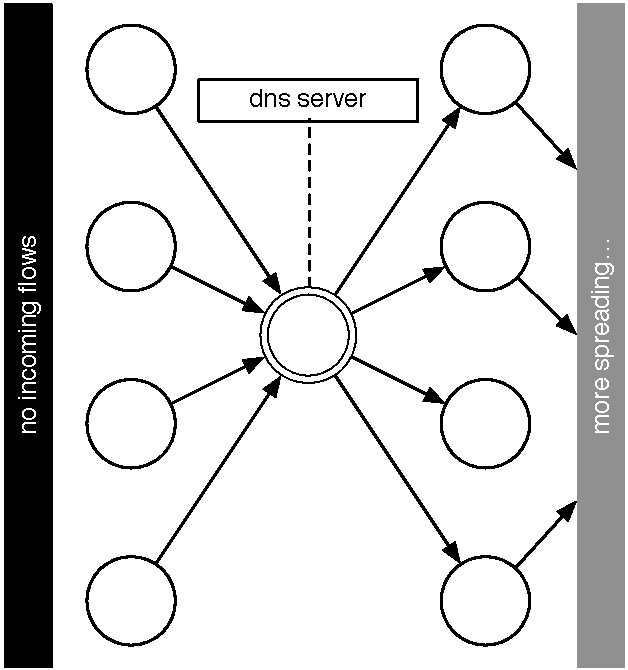
\includegraphics[width=0.5\textwidth]{dns-clients}
\end{figure}

By having the possibility to exclude vertices with few clients from the end results,
 it is trivial to limit the results to vertices with the second-longest path.
This will make it easier to focus on hosts that forward traffic, and not on hosts that only initiate traffic.

